\documentclass{scrartcl}
\usepackage[a4paper,left=1in,right=1in,top=1.2in,bottom=1in]{geometry}
\usepackage{siunitx}
\usepackage{graphicx}
\setkomafont{disposition}{\normalfont\bfseries}
\usepackage{amsmath}
\usepackage{lipsum}
\allowdisplaybreaks

%title
\title{Extra assignment:\\Inference for continuous detection and discrimination}
\subtitle{Theoretical Neuroscience II}
\author{Johannes G\"atjen}


\begin{document}
\maketitle

\section{Theoretical maximum density}

\begin{align*}
r_k =& c_s \exp{(2 \cos{\theta_k-\theta_s)}}\\
\ln{\operatorname{p}(x_k, c_s, \theta_s)} =& 
	\ln{\frac{\pi}{2} + 
	\ln{x_k} - 
	2 \ln{r_k} - 
	\frac{\pi x_k^2}{4r_k^2} -
	\ln{2\pi} - 
	\frac{c_s}{c_0} - 
	\ln{c_0}}\\	
\operatorname{p} (x_k, c_s, \theta_s) =& 
	\frac{x_k r_k}{4 c_0} \cdot 
	\exp{\left( 
		-\frac{\pi x_k^2}{4r_k^2} - 
		\frac{c_s}{c_0} - 2 
		\right)}\\	
0 = \frac{\partial \operatorname{p} (x_k, c_s, \theta_s)}{\partial x_k} =& 
	\frac{r_k}{4c_0} 
	\exp{\left( 
		-x_k^2 
		\frac{\pi}{4r_k^2} - 
		\frac{c_s}{c_0} - 2 
		\right)} + 
	\frac{x_k r_k}{4c_0}
	\frac{-2\pi x_k}{4r_k^2} 
	\exp{\left( 
		-x_k^2 
		\frac{\pi}{4r_k^2} 
		\right) }\\	
=& \underbrace{
		\exp{\left( 
			-x_k^2 
			\frac{\pi}{4r_k^2}  
			\right)}
		\frac{r_k}{4c_0}}_{\neq 0} \cdot 
	\left( 1 - 2\pi x_k^2 \right)\\
x_k^2 =& \frac{1}{2\pi}\\
x_k =& \sqrt{\frac{1}{2\pi}}\\ \\
\operatorname{p}(\sqrt{1/2\pi}, c_s, \theta_s) =& 
	\frac{c_s 
		\exp{\left( 
			2 \cos{\theta_k - \theta_s}
			\right)}}
		{4c_0\sqrt{2\pi}} \cdot
	 \exp{\left(
	 	-\frac{1}{8c_s}
	 	\exp{\left(
	 		-2\cos{\theta_k - \theta_s}
	 		\right)}-
	 	\frac{c_s}{c_0}-2
	 	\right)} \\	 	
0 = \frac{\partial \operatorname{p}(\sqrt{1/2\pi}, c_s, \theta_s)}{\partial \theta_s} =& \exp{\left(
		-\frac{1}{8c_s}
		\exp{\left(
			-2\cos{\theta_k - \theta_s}
			\right)} -
		\frac{c_s}{c_0}-2
		\right)} \cdot \\
	&\frac{c_s 
		\exp{\left(
			2 \cos{\theta_k - \theta_s}
			\right)}}
		{4c_0\sqrt{2\pi}} 
	\frac{2\sin{\theta_k-\theta_s}}{8c_s\exp{\left(
		2\cos{\theta_k - \theta_s}
		\right)}} \\
+& \exp{\left(
		-\frac{1}{8c_s}
		\exp{\left(
			-2\cos{\theta_k - \theta_s}
			\right)} -
		\frac{c_s}{c_0}-2
		\right)} \cdot \\
	 &\exp{\left(
	 	2\cos{\theta_k - \theta_s}
	 	\right)} 
	 \frac{2c_s\sin{\theta_k-\theta_s}}{4c_0\sqrt{2\pi}} \\
=& \underbrace{\exp{\left(
		-\frac{1}{8c_s}
		\exp{\left(
			-2\cos{\theta_k - \theta_s}
			\right)} -
		\frac{c_s}{c_0}-2
		\right)}
	\exp{(2\cos{\theta_k-\theta_s})}
	\frac{2c_s}{4c_0\sqrt{2\pi}}}_{\neq 0} \cdot \\
	&\sin{(\theta_k-\theta_s)}
	\underbrace{\left(
		\frac{1}{8c_s} \exp{(-2\cos{(\theta_k-\theta_s)})}
		+1
		\right)}_{\neq 0}\\
0 =& \sin{\theta_k - \theta_s} \\
\theta_s =& \theta_k \\ \\
\operatorname{p}(\sqrt{1/2\pi}, c_s, \theta_k) =& \frac{c_s e^2}{4c_0 \sqrt{2\pi}}
	\exp{\left(
		-\frac{1}{8c_se^2} - 
		\frac{c_s}{c_0} - 2
		\right)} \\
0 = \frac{\partial \operatorname{p}(\sqrt{1/2\pi}, c_s, \theta_k)}{\partial c_s} =& 
	\frac{c_s e^2}{4c_0 \sqrt{2\pi}}
	\exp{\left(
		-\frac{1}{8c_se^2} - 
		\frac{c_s}{c_0} - 2
		\right)}
	\left(
		-\frac{1}{c_0}
		+ \frac{1}{8c_s^2e^2}
		\right)	\\
	+& \exp{\left(
		-\frac{1}{8c_se^2} - 
		\frac{c_s}{c_0} - 2
		\right)}
	\frac{e^2}{4c_0\sqrt{2\pi}} \\
=& \underbrace{\left(
	\exp{\left(
		-\frac{1}{8c_se^2} - 
		\frac{c_s}{c_0} - 2
		\right)}
	\frac{e^2}{4c_s\sqrt{2\pi}}
	\right)}_{\neq 0} \cdot
	\left(
		\frac{1}{8c_se^2} - \frac{c_s}{c_0} + 1
		\right)\\
0 =& c_s^2 - c_sc_0 - \frac{c_0}{8e^2} \\
c_s =& \frac{c_0}{2} +
	\sqrt{
		\frac{c_0^2}{4}+
		\frac{c_0}{8e^2}}
\end{align*}

\lipsum
%include picture
%\begin{figure}[h]
%\centering
%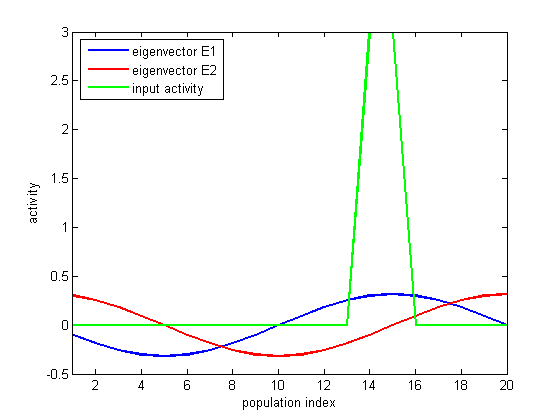
\includegraphics[trim = {0.6cm 0 1.2cm 0.7cm}, width=0.7\textwidth, clip]{../pics/eigen}
%\caption{Visualization of network connectivity eigenvectors (red and blue) and an example input (green), as a function of population index.}
%\label{label}
%\end{figure}


\end{document}